\documentclass[1p]{elsarticle_modified}
%\bibliographystyle{elsarticle-num}

%\usepackage[colorlinks]{hyperref}
%\usepackage{abbrmath_seonhwa} %\Abb, \Ascr, \Acal ,\Abf, \Afrak
\usepackage{amsfonts}
\usepackage{amssymb}
\usepackage{amsmath}
\usepackage{amsthm}
\usepackage{scalefnt}
\usepackage{amsbsy}
\usepackage{kotex}
\usepackage{caption}
\usepackage{subfig}
\usepackage{color}
\usepackage{graphicx}
\usepackage{xcolor} %% white, black, red, green, blue, cyan, magenta, yellow
\usepackage{float}
\usepackage{setspace}
\usepackage{hyperref}

\usepackage{tikz}
\usetikzlibrary{arrows}

\usepackage{multirow}
\usepackage{array} % fixed length table
\usepackage{hhline}

%%%%%%%%%%%%%%%%%%%%%
\makeatletter
\renewcommand*\env@matrix[1][\arraystretch]{%
	\edef\arraystretch{#1}%
	\hskip -\arraycolsep
	\let\@ifnextchar\new@ifnextchar
	\array{*\c@MaxMatrixCols c}}
\makeatother %https://tex.stackexchange.com/questions/14071/how-can-i-increase-the-line-spacing-in-a-matrix
%%%%%%%%%%%%%%%

\usepackage[normalem]{ulem}

\newcommand{\msout}[1]{\ifmmode\text{\sout{\ensuremath{#1}}}\else\sout{#1}\fi}
%SOURCE: \msout is \stkout macro in https://tex.stackexchange.com/questions/20609/strikeout-in-math-mode

\newcommand{\cancel}[1]{
	\ifmmode
	{\color{red}\msout{#1}}
	\else
	{\color{red}\sout{#1}}
	\fi
}

\newcommand{\add}[1]{
	{\color{blue}\uwave{#1}}
}

\newcommand{\replace}[2]{
	\ifmmode
	{\color{red}\msout{#1}}{\color{blue}\uwave{#2}}
	\else
	{\color{red}\sout{#1}}{\color{blue}\uwave{#2}}
	\fi
}

\newcommand{\Sol}{\mathcal{S}} %segment
\newcommand{\D}{D} %diagram
\newcommand{\A}{\mathcal{A}} %arc


%%%%%%%%%%%%%%%%%%%%%%%%%%%%%5 test

\def\sl{\operatorname{\textup{SL}}(2,\Cbb)}
\def\psl{\operatorname{\textup{PSL}}(2,\Cbb)}
\def\quan{\mkern 1mu \triangleright \mkern 1mu}

\theoremstyle{definition}
\newtheorem{thm}{Theorem}[section]
\newtheorem{prop}[thm]{Proposition}
\newtheorem{lem}[thm]{Lemma}
\newtheorem{ques}[thm]{Question}
\newtheorem{cor}[thm]{Corollary}
\newtheorem{defn}[thm]{Definition}
\newtheorem{exam}[thm]{Example}
\newtheorem{rmk}[thm]{Remark}
\newtheorem{alg}[thm]{Algorithm}

\newcommand{\I}{\sqrt{-1}}
\begin{document}

%\begin{frontmatter}
%
%\title{Boundary parabolic representations of knots up to 8 crossings}
%
%%% Group authors per affiliation:
%\author{Yunhi Cho} 
%\address{Department of Mathematics, University of Seoul, Seoul, Korea}
%\ead{yhcho@uos.ac.kr}
%
%
%\author{Seonhwa Kim} %\fnref{s_kim}}
%\address{Center for Geometry and Physics, Institute for Basic Science, Pohang, 37673, Korea}
%\ead{ryeona17@ibs.re.kr}
%
%\author{Hyuk Kim}
%\address{Department of Mathematical Sciences, Seoul National University, Seoul 08826, Korea}
%\ead{hyukkim@snu.ac.kr}
%
%\author{Seokbeom Yoon}
%\address{Department of Mathematical Sciences, Seoul National University, Seoul, 08826,  Korea}
%\ead{sbyoon15@snu.ac.kr}
%
%\begin{abstract}
%We find all boundary parabolic representation of knots up to 8 crossings.
%
%\end{abstract}
%\begin{keyword}
%    \MSC[2010] 57M25 
%\end{keyword}
%
%\end{frontmatter}

%\linenumbers
%\tableofcontents
%
\newcommand\colored[1]{\textcolor{white}{\rule[-0.35ex]{0.8em}{1.4ex}}\kern-0.8em\color{red} #1}%
%\newcommand\colored[1]{\textcolor{white}{ #1}\kern-2.17ex	\textcolor{white}{ #1}\kern-1.81ex	\textcolor{white}{ #1}\kern-2.15ex\color{red}#1	}

{\Large $\underline{12n_{0515}~(K12n_{0515})}$}

\setlength{\tabcolsep}{10pt}
\renewcommand{\arraystretch}{1.6}
\vspace{1cm}\begin{tabular}{m{100pt}>{\centering\arraybackslash}m{274pt}}
\multirow{5}{120pt}{
	\centering
	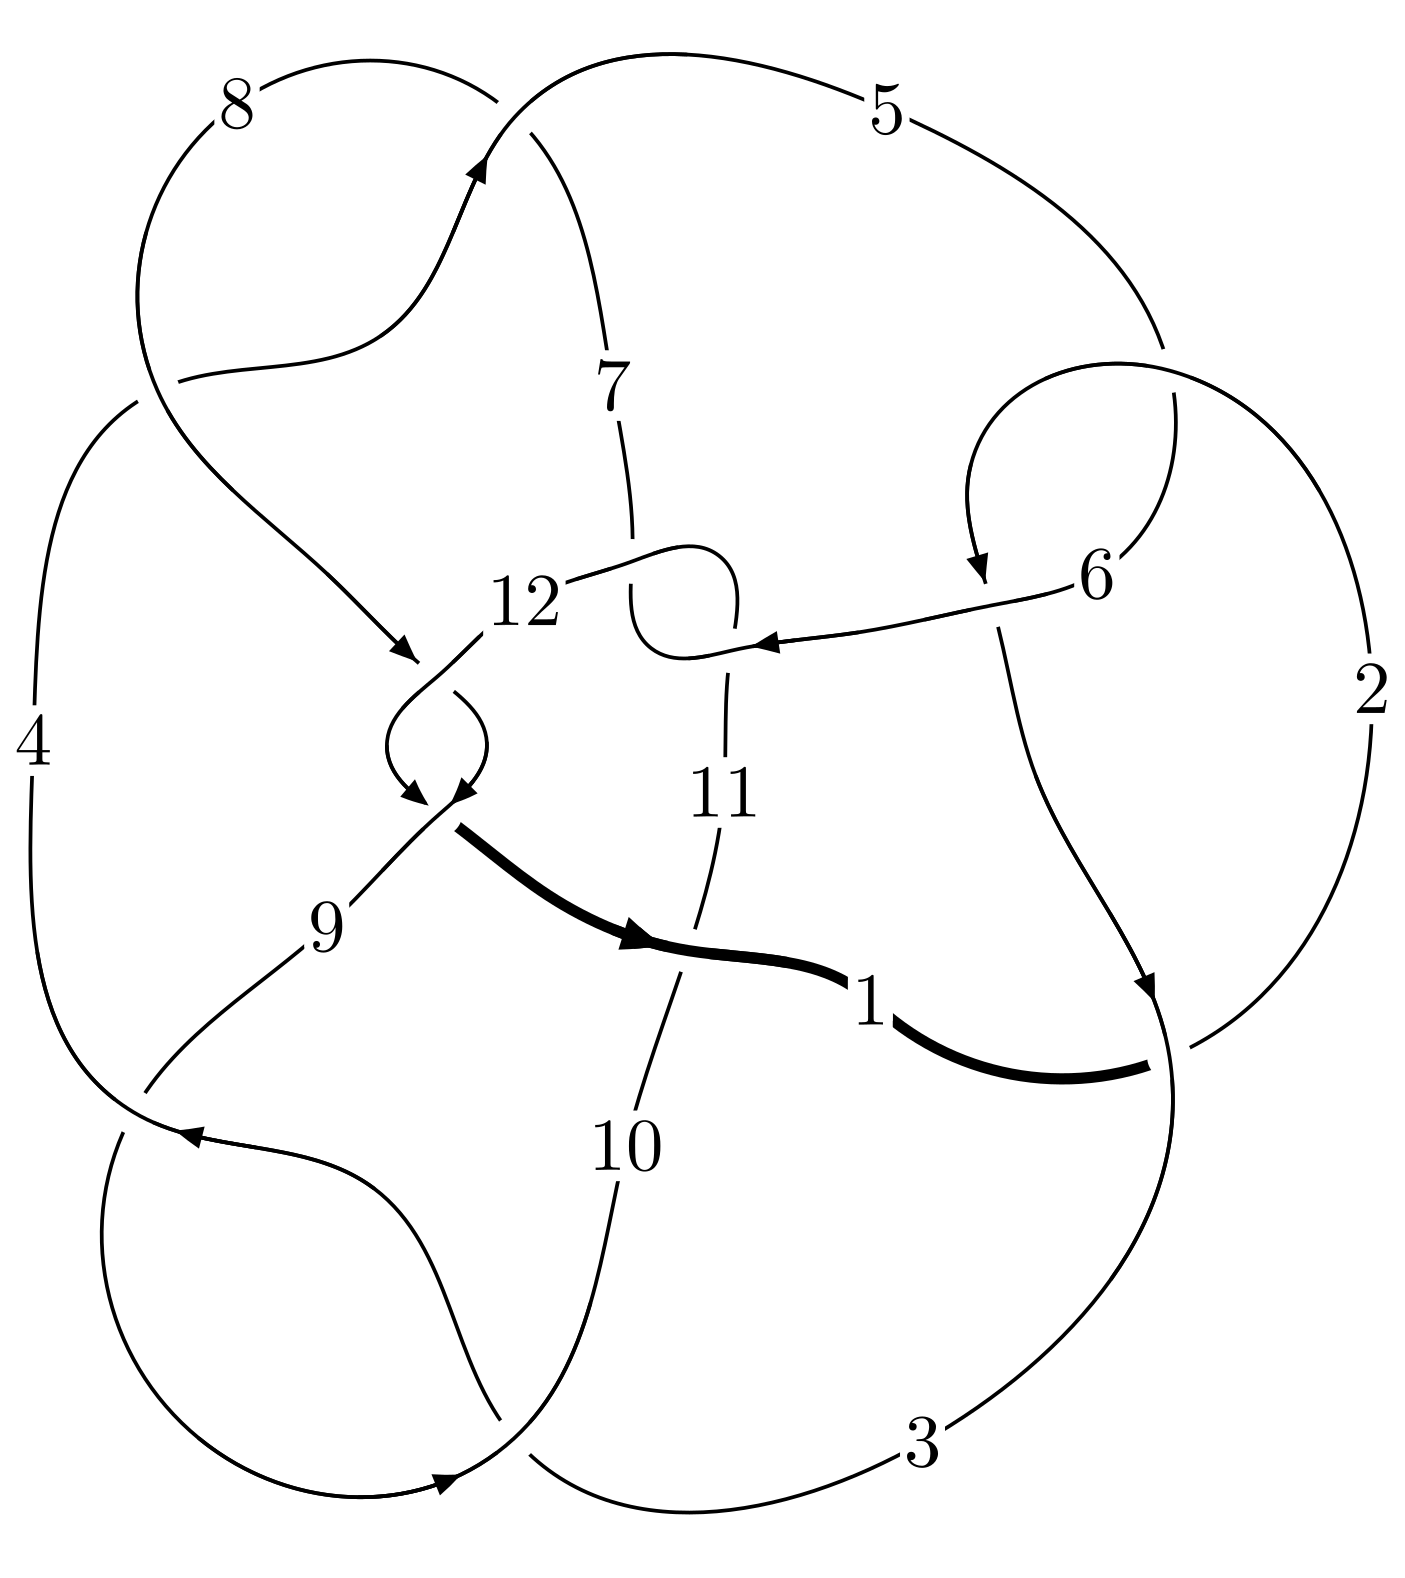
\includegraphics[width=112pt]{../../../GIT/diagram.site/Diagrams/png/2604_12n_0515.png}\\
\ \ \ A knot diagram\footnotemark}&
\allowdisplaybreaks
\textbf{Linearized knot diagam} \\
\cline{2-2}
 &
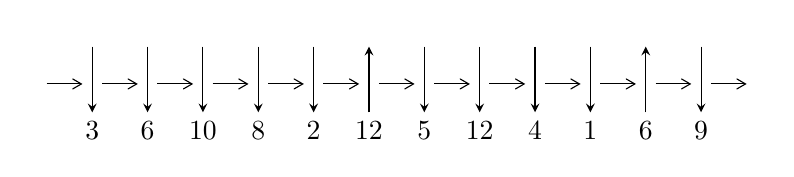
\begin{tikzpicture}[x=20pt, y=17pt]
	% nodes
	\node (C0) at (0, 0) {};
	\node (C1) at (1, 0) {};
	\node (C1U) at (1, +1) {};
	\node (C1D) at (1, -1) {3};

	\node (C2) at (2, 0) {};
	\node (C2U) at (2, +1) {};
	\node (C2D) at (2, -1) {6};

	\node (C3) at (3, 0) {};
	\node (C3U) at (3, +1) {};
	\node (C3D) at (3, -1) {10};

	\node (C4) at (4, 0) {};
	\node (C4U) at (4, +1) {};
	\node (C4D) at (4, -1) {8};

	\node (C5) at (5, 0) {};
	\node (C5U) at (5, +1) {};
	\node (C5D) at (5, -1) {2};

	\node (C6) at (6, 0) {};
	\node (C6U) at (6, +1) {};
	\node (C6D) at (6, -1) {12};

	\node (C7) at (7, 0) {};
	\node (C7U) at (7, +1) {};
	\node (C7D) at (7, -1) {5};

	\node (C8) at (8, 0) {};
	\node (C8U) at (8, +1) {};
	\node (C8D) at (8, -1) {12};

	\node (C9) at (9, 0) {};
	\node (C9U) at (9, +1) {};
	\node (C9D) at (9, -1) {4};

	\node (C10) at (10, 0) {};
	\node (C10U) at (10, +1) {};
	\node (C10D) at (10, -1) {1};

	\node (C11) at (11, 0) {};
	\node (C11U) at (11, +1) {};
	\node (C11D) at (11, -1) {6};

	\node (C12) at (12, 0) {};
	\node (C12U) at (12, +1) {};
	\node (C12D) at (12, -1) {9};
	\node (C13) at (13, 0) {};

	% arrows
	\draw[->,>={angle 60}]
	(C0) edge (C1) (C1) edge (C2) (C2) edge (C3) (C3) edge (C4) (C4) edge (C5) (C5) edge (C6) (C6) edge (C7) (C7) edge (C8) (C8) edge (C9) (C9) edge (C10) (C10) edge (C11) (C11) edge (C12) (C12) edge (C13) ;	\draw[->,>=stealth]
	(C1U) edge (C1D) (C2U) edge (C2D) (C3U) edge (C3D) (C4U) edge (C4D) (C5U) edge (C5D) (C6D) edge (C6U) (C7U) edge (C7D) (C8U) edge (C8D) (C9U) edge (C9D) (C10U) edge (C10D) (C11D) edge (C11U) (C12U) edge (C12D) ;
	\end{tikzpicture} \\
\hhline{~~} \\& 
\textbf{Solving Sequence} \\ \cline{2-2} 
 &
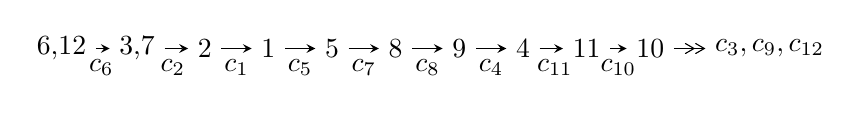
\begin{tikzpicture}[x=23pt, y=7pt]
	% node
	\node (A0) at (-1/8, 0) {6,12};
	\node (A1) at (17/16, 0) {3,7};
	\node (A2) at (17/8, 0) {2};
	\node (A3) at (25/8, 0) {1};
	\node (A4) at (33/8, 0) {5};
	\node (A5) at (41/8, 0) {8};
	\node (A6) at (49/8, 0) {9};
	\node (A7) at (57/8, 0) {4};
	\node (A8) at (65/8, 0) {11};
	\node (A9) at (73/8, 0) {10};
	\node (C1) at (1/2, -1) {$c_{6}$};
	\node (C2) at (13/8, -1) {$c_{2}$};
	\node (C3) at (21/8, -1) {$c_{1}$};
	\node (C4) at (29/8, -1) {$c_{5}$};
	\node (C5) at (37/8, -1) {$c_{7}$};
	\node (C6) at (45/8, -1) {$c_{8}$};
	\node (C7) at (53/8, -1) {$c_{4}$};
	\node (C8) at (61/8, -1) {$c_{11}$};
	\node (C9) at (69/8, -1) {$c_{10}$};
	\node (A10) at (11, 0) {$c_{3},c_{9},c_{12}$};

	% edge
	\draw[->,>=stealth]	
	(A0) edge (A1) (A1) edge (A2) (A2) edge (A3) (A3) edge (A4) (A4) edge (A5) (A5) edge (A6) (A6) edge (A7) (A7) edge (A8) (A8) edge (A9) ;
	\draw[->>,>={angle 60}]	
	(A9) edge (A10);
\end{tikzpicture} \\ 

\end{tabular} \\

\footnotetext{
The image of knot diagram is generated by the software ``\textbf{Draw programme}" developed by Andrew Bartholomew(\url{http://www.layer8.co.uk/maths/draw/index.htm\#Running-draw}), where we modified some parts for our purpose(\url{https://github.com/CATsTAILs/LinksPainter}).
}\phantom \\ \newline 
\centering \textbf{Ideals for irreducible components\footnotemark of $X_{\text{par}}$} 
 
\begin{align*}
I^u_{1}&=\langle 
8.22266\times10^{274} u^{59}-2.15506\times10^{275} u^{58}+\cdots+2.34069\times10^{278} b-6.04308\times10^{278},\\
\phantom{I^u_{1}}&\phantom{= \langle  }1.35060\times10^{279} u^{59}-3.78638\times10^{279} u^{58}+\cdots+8.33051\times10^{281} a-1.96121\times10^{283},\\
\phantom{I^u_{1}}&\phantom{= \langle  }u^{60}-3 u^{59}+\cdots-11482 u+3559\rangle \\
I^u_{2}&=\langle 
-14967763 u^{15}-2907851 u^{14}+\cdots+25980989 b+31360586,\\
\phantom{I^u_{2}}&\phantom{= \langle  }50615010 u^{15}+19279984 u^{14}+\cdots+25980989 a-107875259,\\
\phantom{I^u_{2}}&\phantom{= \langle  }u^{16}+2 u^{14}-4 u^{13}-6 u^{12}-4 u^{11}+5 u^{10}+8 u^9+28 u^8-32 u^7+25 u^6-51 u^5+36 u^4-15 u^3+13 u^2-6 u+1\rangle \\
\\
\end{align*}
\raggedright * 2 irreducible components of $\dim_{\mathbb{C}}=0$, with total 76 representations.\\
\footnotetext{All coefficients of polynomials are rational numbers. But the coefficients are sometimes approximated in decimal forms when there is not enough margin.}
\newpage
\renewcommand{\arraystretch}{1}
\centering \section*{I. $I^u_{1}= \langle 8.22\times10^{274} u^{59}-2.16\times10^{275} u^{58}+\cdots+2.34\times10^{278} b-6.04\times10^{278},\;1.35\times10^{279} u^{59}-3.79\times10^{279} u^{58}+\cdots+8.33\times10^{281} a-1.96\times10^{283},\;u^{60}-3 u^{59}+\cdots-11482 u+3559 \rangle$}
\flushleft \textbf{(i) Arc colorings}\\
\begin{tabular}{m{7pt} m{180pt} m{7pt} m{180pt} }
\flushright $a_{6}=$&$\begin{pmatrix}1\\0\end{pmatrix}$ \\
\flushright $a_{12}=$&$\begin{pmatrix}0\\u\end{pmatrix}$ \\
\flushright $a_{3}=$&$\begin{pmatrix}-0.00162127 u^{59}+0.00454519 u^{58}+\cdots+14.3091 u+23.5425\\-0.000351292 u^{59}+0.000920694 u^{58}+\cdots-5.50751 u+2.58176\end{pmatrix}$ \\
\flushright $a_{7}=$&$\begin{pmatrix}1\\- u^2\end{pmatrix}$ \\
\flushright $a_{2}=$&$\begin{pmatrix}-0.00197256 u^{59}+0.00546589 u^{58}+\cdots+8.80155 u+26.1243\\-0.000351292 u^{59}+0.000920694 u^{58}+\cdots-5.50751 u+2.58176\end{pmatrix}$ \\
\flushright $a_{1}=$&$\begin{pmatrix}-0.000985855 u^{59}+0.00264770 u^{58}+\cdots-12.7756 u+10.9512\\0.0000228831 u^{59}-0.000129239 u^{58}+\cdots-3.83757 u-1.50813\end{pmatrix}$ \\
\flushright $a_{5}=$&$\begin{pmatrix}-0.00191681 u^{59}+0.00522142 u^{58}+\cdots+7.64525 u+28.4871\\-0.000498029 u^{59}+0.00130545 u^{58}+\cdots-1.84746 u+4.50416\end{pmatrix}$ \\
\flushright $a_{8}=$&$\begin{pmatrix}-0.00166805 u^{59}+0.00435306 u^{58}+\cdots-14.8874 u+11.7806\\0.000432015 u^{59}-0.00114140 u^{58}+\cdots-0.328575 u-5.15749\end{pmatrix}$ \\
\flushright $a_{9}=$&$\begin{pmatrix}-0.00166805 u^{59}+0.00435306 u^{58}+\cdots-14.8874 u+11.7806\\0.000199584 u^{59}-0.000526762 u^{58}+\cdots-1.86786 u-2.84024\end{pmatrix}$ \\
\flushright $a_{4}=$&$\begin{pmatrix}-0.000752232 u^{59}+0.00207616 u^{58}+\cdots+1.48938 u+14.5021\\-0.000400020 u^{59}+0.00107306 u^{58}+\cdots+0.385314 u+4.95029\end{pmatrix}$ \\
\flushright $a_{11}=$&$\begin{pmatrix}- u\\u\end{pmatrix}$ \\
\flushright $a_{10}=$&$\begin{pmatrix}0.00242528 u^{59}-0.00649531 u^{58}+\cdots+11.3474 u-23.9948\\0.000228355 u^{59}-0.000590475 u^{58}+\cdots+7.46556 u-2.03457\end{pmatrix}$\\&\end{tabular}
\flushleft \textbf{(ii) Obstruction class $= -1$}\\~\\
\flushleft \textbf{(iii) Cusp Shapes $= 0.00130054 u^{59}-0.00350454 u^{58}+\cdots-11.7943 u-31.3032$}\\~\\
\newpage\renewcommand{\arraystretch}{1}
\flushleft \textbf{(iv) u-Polynomials at the component}\newline \\
\begin{tabular}{m{50pt}|m{274pt}}
Crossings & \hspace{64pt}u-Polynomials at each crossing \\
\hline $$\begin{aligned}c_{1}\end{aligned}$$&$\begin{aligned}
&u^{60}+35 u^{59}+\cdots+2933 u+361
\end{aligned}$\\
\hline $$\begin{aligned}c_{2},c_{5}\end{aligned}$$&$\begin{aligned}
&u^{60}+u^{59}+\cdots-27 u-19
\end{aligned}$\\
\hline $$\begin{aligned}c_{3},c_{9}\end{aligned}$$&$\begin{aligned}
&u^{60}+u^{59}+\cdots+46 u-43
\end{aligned}$\\
\hline $$\begin{aligned}c_{4},c_{7}\end{aligned}$$&$\begin{aligned}
&u^{60}-4 u^{59}+\cdots-12 u+1
\end{aligned}$\\
\hline $$\begin{aligned}c_{6},c_{11}\end{aligned}$$&$\begin{aligned}
&u^{60}-3 u^{59}+\cdots-11482 u+3559
\end{aligned}$\\
\hline $$\begin{aligned}c_{8},c_{12}\end{aligned}$$&$\begin{aligned}
&u^{60}+3 u^{59}+\cdots+568 u+23
\end{aligned}$\\
\hline $$\begin{aligned}c_{10}\end{aligned}$$&$\begin{aligned}
&u^{60}+u^{59}+\cdots+15055 u-761
\end{aligned}$\\
\hline
\end{tabular}\\~\\
\newpage\renewcommand{\arraystretch}{1}
\flushleft \textbf{(v) Riley Polynomials at the component}\newline \\
\begin{tabular}{m{50pt}|m{274pt}}
Crossings & \hspace{64pt}Riley Polynomials at each crossing \\
\hline $$\begin{aligned}c_{1}\end{aligned}$$&$\begin{aligned}
&y^{60}-11 y^{59}+\cdots-3170161 y+130321
\end{aligned}$\\
\hline $$\begin{aligned}c_{2},c_{5}\end{aligned}$$&$\begin{aligned}
&y^{60}-35 y^{59}+\cdots-2933 y+361
\end{aligned}$\\
\hline $$\begin{aligned}c_{3},c_{9}\end{aligned}$$&$\begin{aligned}
&y^{60}+49 y^{59}+\cdots+10526 y+1849
\end{aligned}$\\
\hline $$\begin{aligned}c_{4},c_{7}\end{aligned}$$&$\begin{aligned}
&y^{60}+2 y^{59}+\cdots-46 y+1
\end{aligned}$\\
\hline $$\begin{aligned}c_{6},c_{11}\end{aligned}$$&$\begin{aligned}
&y^{60}+65 y^{59}+\cdots-502242808 y+12666481
\end{aligned}$\\
\hline $$\begin{aligned}c_{8},c_{12}\end{aligned}$$&$\begin{aligned}
&y^{60}-47 y^{59}+\cdots-56882 y+529
\end{aligned}$\\
\hline $$\begin{aligned}c_{10}\end{aligned}$$&$\begin{aligned}
&y^{60}-23 y^{59}+\cdots-95786899 y+579121
\end{aligned}$\\
\hline
\end{tabular}\\~\\
\newpage\flushleft \textbf{(vi) Complex Volumes and Cusp Shapes}
$$\begin{array}{c|c|c}  
\text{Solutions to }I^u_{1}& \I (\text{vol} + \sqrt{-1}CS) & \text{Cusp shape}\\
 \hline 
\begin{aligned}
u &= -1.007350 + 0.006718 I \\
a &= -0.051105 - 0.783732 I \\
b &= -0.856821 + 0.663890 I\end{aligned}
 & \phantom{-}8.73644 + 2.57827 I & \phantom{-}3.69883 - 3.02158 I \\ \hline\begin{aligned}
u &= -1.007350 - 0.006718 I \\
a &= -0.051105 + 0.783732 I \\
b &= -0.856821 - 0.663890 I\end{aligned}
 & \phantom{-}8.73644 - 2.57827 I & \phantom{-}3.69883 + 3.02158 I \\ \hline\begin{aligned}
u &= \phantom{-}0.167317 + 1.021400 I \\
a &= -0.69860 - 1.40758 I \\
b &= \phantom{-}0.176226 + 0.887745 I\end{aligned}
 & \phantom{-}3.79265 - 1.97736 I & \phantom{-}0.36666 + 2.76154 I \\ \hline\begin{aligned}
u &= \phantom{-}0.167317 - 1.021400 I \\
a &= -0.69860 + 1.40758 I \\
b &= \phantom{-}0.176226 - 0.887745 I\end{aligned}
 & \phantom{-}3.79265 + 1.97736 I & \phantom{-}0.36666 - 2.76154 I \\ \hline\begin{aligned}
u &= \phantom{-}0.120119 + 0.949857 I \\
a &= \phantom{-}0.243764 - 0.379978 I \\
b &= \phantom{-}0.032250 + 0.520457 I\end{aligned}
 & -0.77619 + 1.28470 I & -6.96269 - 5.03629 I \\ \hline\begin{aligned}
u &= \phantom{-}0.120119 - 0.949857 I \\
a &= \phantom{-}0.243764 + 0.379978 I \\
b &= \phantom{-}0.032250 - 0.520457 I\end{aligned}
 & -0.77619 - 1.28470 I & -6.96269 + 5.03629 I \\ \hline\begin{aligned}
u &= -0.436643 + 0.834573 I \\
a &= \phantom{-}0.916522 + 0.292944 I \\
b &= -0.973516 + 0.318596 I\end{aligned}
 & -0.52721 - 1.87425 I & -8.40865 + 2.07235 I \\ \hline\begin{aligned}
u &= -0.436643 - 0.834573 I \\
a &= \phantom{-}0.916522 - 0.292944 I \\
b &= -0.973516 - 0.318596 I\end{aligned}
 & -0.52721 + 1.87425 I & -8.40865 - 2.07235 I \\ \hline\begin{aligned}
u &= \phantom{-}0.233820 + 1.070940 I \\
a &= -0.287355 - 0.183543 I \\
b &= \phantom{-}0.439508 + 0.589156 I\end{aligned}
 & -0.817883 + 0.949182 I & -8.00000 + 0. I\phantom{ +0.000000I} \\ \hline\begin{aligned}
u &= \phantom{-}0.233820 - 1.070940 I \\
a &= -0.287355 + 0.183543 I \\
b &= \phantom{-}0.439508 - 0.589156 I\end{aligned}
 & -0.817883 - 0.949182 I & -8.00000 + 0. I\phantom{ +0.000000I}\\
 \hline 
 \end{array}$$\newpage$$\begin{array}{c|c|c}  
\text{Solutions to }I^u_{1}& \I (\text{vol} + \sqrt{-1}CS) & \text{Cusp shape}\\
 \hline 
\begin{aligned}
u &= -0.783519 + 0.441750 I \\
a &= \phantom{-}1.19806 - 1.78599 I \\
b &= -0.902727 + 1.012570 I\end{aligned}
 & \phantom{-}2.59861 + 3.60251 I & -5.47993 - 4.86448 I \\ \hline\begin{aligned}
u &= -0.783519 - 0.441750 I \\
a &= \phantom{-}1.19806 + 1.78599 I \\
b &= -0.902727 - 1.012570 I\end{aligned}
 & \phantom{-}2.59861 - 3.60251 I & -5.47993 + 4.86448 I \\ \hline\begin{aligned}
u &= -0.346136 + 1.116180 I \\
a &= -0.69410 + 1.24191 I \\
b &= -1.129160 - 0.396009 I\end{aligned}
 & -3.89834 - 2.15588 I & \phantom{-0.000000 } 0 \\ \hline\begin{aligned}
u &= -0.346136 - 1.116180 I \\
a &= -0.69410 - 1.24191 I \\
b &= -1.129160 + 0.396009 I\end{aligned}
 & -3.89834 + 2.15588 I & \phantom{-0.000000 } 0 \\ \hline\begin{aligned}
u &= -1.280030 + 0.312941 I \\
a &= -0.02697 - 1.54626 I \\
b &= \phantom{-}0.907660 + 0.163934 I\end{aligned}
 & \phantom{-}5.59454 - 0.79177 I & \phantom{-0.000000 } 0 \\ \hline\begin{aligned}
u &= -1.280030 - 0.312941 I \\
a &= -0.02697 + 1.54626 I \\
b &= \phantom{-}0.907660 - 0.163934 I\end{aligned}
 & \phantom{-}5.59454 + 0.79177 I & \phantom{-0.000000 } 0 \\ \hline\begin{aligned}
u &= \phantom{-}0.673670 + 0.088043 I \\
a &= -1.13855 + 0.86484 I \\
b &= \phantom{-}1.018250 - 0.455571 I\end{aligned}
 & \phantom{-}1.34053 + 2.69149 I & -4.70869 - 3.74095 I \\ \hline\begin{aligned}
u &= \phantom{-}0.673670 - 0.088043 I \\
a &= -1.13855 - 0.86484 I \\
b &= \phantom{-}1.018250 + 0.455571 I\end{aligned}
 & \phantom{-}1.34053 - 2.69149 I & -4.70869 + 3.74095 I \\ \hline\begin{aligned}
u &= \phantom{-}0.179970 + 1.330630 I \\
a &= \phantom{-}0.613950 + 1.012280 I \\
b &= \phantom{-}1.119500 - 0.531381 I\end{aligned}
 & -2.96619 + 5.50433 I & \phantom{-0.000000 } 0 \\ \hline\begin{aligned}
u &= \phantom{-}0.179970 - 1.330630 I \\
a &= \phantom{-}0.613950 - 1.012280 I \\
b &= \phantom{-}1.119500 + 0.531381 I\end{aligned}
 & -2.96619 - 5.50433 I & \phantom{-0.000000 } 0\\
 \hline 
 \end{array}$$\newpage$$\begin{array}{c|c|c}  
\text{Solutions to }I^u_{1}& \I (\text{vol} + \sqrt{-1}CS) & \text{Cusp shape}\\
 \hline 
\begin{aligned}
u &= \phantom{-}1.342990 + 0.174597 I \\
a &= -0.48406 - 1.61748 I \\
b &= \phantom{-}0.662047 + 0.683351 I\end{aligned}
 & \phantom{-}3.31510 - 2.64385 I & \phantom{-0.000000 } 0 \\ \hline\begin{aligned}
u &= \phantom{-}1.342990 - 0.174597 I \\
a &= -0.48406 + 1.61748 I \\
b &= \phantom{-}0.662047 - 0.683351 I\end{aligned}
 & \phantom{-}3.31510 + 2.64385 I & \phantom{-0.000000 } 0 \\ \hline\begin{aligned}
u &= \phantom{-}0.631122 + 0.052699 I \\
a &= -0.61769 - 1.35412 I \\
b &= \phantom{-}0.921626 + 0.670766 I\end{aligned}
 & \phantom{-}1.60978 - 2.58403 I & -1.183332 - 0.037949 I \\ \hline\begin{aligned}
u &= \phantom{-}0.631122 - 0.052699 I \\
a &= -0.61769 + 1.35412 I \\
b &= \phantom{-}0.921626 - 0.670766 I\end{aligned}
 & \phantom{-}1.60978 + 2.58403 I & -1.183332 + 0.037949 I \\ \hline\begin{aligned}
u &= -0.520152 + 0.044751 I \\
a &= \phantom{-}2.22330 + 0.65037 I \\
b &= -0.529944 - 0.260822 I\end{aligned}
 & -1.347560 + 0.092496 I & -5.86116 + 1.61635 I \\ \hline\begin{aligned}
u &= -0.520152 - 0.044751 I \\
a &= \phantom{-}2.22330 - 0.65037 I \\
b &= -0.529944 + 0.260822 I\end{aligned}
 & -1.347560 - 0.092496 I & -5.86116 - 1.61635 I \\ \hline\begin{aligned}
u &= \phantom{-}0.37351 + 1.47885 I \\
a &= -0.042265 + 0.991284 I \\
b &= \phantom{-}0.254547 - 0.892528 I\end{aligned}
 & -2.44888 - 1.09682 I & \phantom{-0.000000 } 0 \\ \hline\begin{aligned}
u &= \phantom{-}0.37351 - 1.47885 I \\
a &= -0.042265 - 0.991284 I \\
b &= \phantom{-}0.254547 + 0.892528 I\end{aligned}
 & -2.44888 + 1.09682 I & \phantom{-0.000000 } 0 \\ \hline\begin{aligned}
u &= \phantom{-}0.379838 + 0.129064 I \\
a &= -2.69838 - 0.75915 I \\
b &= \phantom{-}0.310209 - 0.552194 I\end{aligned}
 & \phantom{-}2.41343 - 4.02201 I & -2.17904 + 4.26768 I \\ \hline\begin{aligned}
u &= \phantom{-}0.379838 - 0.129064 I \\
a &= -2.69838 + 0.75915 I \\
b &= \phantom{-}0.310209 + 0.552194 I\end{aligned}
 & \phantom{-}2.41343 + 4.02201 I & -2.17904 - 4.26768 I\\
 \hline 
 \end{array}$$\newpage$$\begin{array}{c|c|c}  
\text{Solutions to }I^u_{1}& \I (\text{vol} + \sqrt{-1}CS) & \text{Cusp shape}\\
 \hline 
\begin{aligned}
u &= -0.342835\phantom{ +0.000000I} \\
a &= \phantom{-}1.82728\phantom{ +0.000000I} \\
b &= -0.751050\phantom{ +0.000000I}\end{aligned}
 & -0.992150\phantom{ +0.000000I} & -10.3910\phantom{ +0.000000I} \\ \hline\begin{aligned}
u &= -0.45172 + 1.60124 I \\
a &= -0.073209 + 1.127150 I \\
b &= \phantom{-}0.012328 - 0.990813 I\end{aligned}
 & -6.51294 - 4.15782 I & \phantom{-0.000000 } 0 \\ \hline\begin{aligned}
u &= -0.45172 - 1.60124 I \\
a &= -0.073209 - 1.127150 I \\
b &= \phantom{-}0.012328 + 0.990813 I\end{aligned}
 & -6.51294 + 4.15782 I & \phantom{-0.000000 } 0 \\ \hline\begin{aligned}
u &= \phantom{-}0.296399 + 0.062088 I \\
a &= \phantom{-}1.87004 - 4.59300 I \\
b &= -0.931163 - 0.266156 I\end{aligned}
 & -2.29321 - 2.81632 I & -7.40161 + 5.36260 I \\ \hline\begin{aligned}
u &= \phantom{-}0.296399 - 0.062088 I \\
a &= \phantom{-}1.87004 + 4.59300 I \\
b &= -0.931163 + 0.266156 I\end{aligned}
 & -2.29321 + 2.81632 I & -7.40161 - 5.36260 I \\ \hline\begin{aligned}
u &= -0.171614 + 0.220877 I \\
a &= -0.57331 - 3.91406 I \\
b &= \phantom{-}1.079170 - 0.455056 I\end{aligned}
 & \phantom{-}0.20500 + 8.08474 I & -6.89819 - 9.56475 I \\ \hline\begin{aligned}
u &= -0.171614 - 0.220877 I \\
a &= -0.57331 + 3.91406 I \\
b &= \phantom{-}1.079170 + 0.455056 I\end{aligned}
 & \phantom{-}0.20500 - 8.08474 I & -6.89819 + 9.56475 I \\ \hline\begin{aligned}
u &= -1.72762\phantom{ +0.000000I} \\
a &= -0.420167\phantom{ +0.000000I} \\
b &= \phantom{-}1.16186\phantom{ +0.000000I}\end{aligned}
 & -5.68066\phantom{ +0.000000I} & \phantom{-0.000000 } 0 \\ \hline\begin{aligned}
u &= \phantom{-}0.13406 + 1.78859 I \\
a &= -0.020787 - 1.023100 I \\
b &= \phantom{-}1.223600 + 0.590393 I\end{aligned}
 & -5.36689 - 6.58267 I & \phantom{-0.000000 } 0 \\ \hline\begin{aligned}
u &= \phantom{-}0.13406 - 1.78859 I \\
a &= -0.020787 + 1.023100 I \\
b &= \phantom{-}1.223600 - 0.590393 I\end{aligned}
 & -5.36689 + 6.58267 I & \phantom{-0.000000 } 0\\
 \hline 
 \end{array}$$\newpage$$\begin{array}{c|c|c}  
\text{Solutions to }I^u_{1}& \I (\text{vol} + \sqrt{-1}CS) & \text{Cusp shape}\\
 \hline 
\begin{aligned}
u &= \phantom{-}0.54349 + 1.71557 I \\
a &= \phantom{-}0.182247 + 1.206790 I \\
b &= -0.223941 - 1.051210 I\end{aligned}
 & -2.29420 + 9.43598 I & \phantom{-0.000000 } 0 \\ \hline\begin{aligned}
u &= \phantom{-}0.54349 - 1.71557 I \\
a &= \phantom{-}0.182247 - 1.206790 I \\
b &= -0.223941 + 1.051210 I\end{aligned}
 & -2.29420 - 9.43598 I & \phantom{-0.000000 } 0 \\ \hline\begin{aligned}
u &= \phantom{-}0.36459 + 1.77723 I \\
a &= -0.882179 - 0.158077 I \\
b &= -0.848721 - 0.077580 I\end{aligned}
 & \phantom{-}0.50904 - 3.72563 I & \phantom{-0.000000 } 0 \\ \hline\begin{aligned}
u &= \phantom{-}0.36459 - 1.77723 I \\
a &= -0.882179 + 0.158077 I \\
b &= -0.848721 + 0.077580 I\end{aligned}
 & \phantom{-}0.50904 + 3.72563 I & \phantom{-0.000000 } 0 \\ \hline\begin{aligned}
u &= \phantom{-}0.96428 + 1.53998 I \\
a &= -0.035444 - 1.020920 I \\
b &= -1.264660 + 0.346449 I\end{aligned}
 & -7.16461 + 2.87399 I & \phantom{-0.000000 } 0 \\ \hline\begin{aligned}
u &= \phantom{-}0.96428 - 1.53998 I \\
a &= -0.035444 + 1.020920 I \\
b &= -1.264660 - 0.346449 I\end{aligned}
 & -7.16461 - 2.87399 I & \phantom{-0.000000 } 0 \\ \hline\begin{aligned}
u &= \phantom{-}0.22234 + 1.88376 I \\
a &= \phantom{-}0.101412 + 0.495797 I \\
b &= \phantom{-}1.213340 - 0.305461 I\end{aligned}
 & -4.20439 + 4.30937 I & \phantom{-0.000000 } 0 \\ \hline\begin{aligned}
u &= \phantom{-}0.22234 - 1.88376 I \\
a &= \phantom{-}0.101412 - 0.495797 I \\
b &= \phantom{-}1.213340 + 0.305461 I\end{aligned}
 & -4.20439 - 4.30937 I & \phantom{-0.000000 } 0 \\ \hline\begin{aligned}
u &= \phantom{-}1.67961 + 0.89723 I \\
a &= \phantom{-}0.479659 + 0.380032 I \\
b &= -1.148550 - 0.220866 I\end{aligned}
 & -1.59063 - 4.29713 I & \phantom{-0.000000 } 0 \\ \hline\begin{aligned}
u &= \phantom{-}1.67961 - 0.89723 I \\
a &= \phantom{-}0.479659 - 0.380032 I \\
b &= -1.148550 + 0.220866 I\end{aligned}
 & -1.59063 + 4.29713 I & \phantom{-0.000000 } 0\\
 \hline 
 \end{array}$$\newpage$$\begin{array}{c|c|c}  
\text{Solutions to }I^u_{1}& \I (\text{vol} + \sqrt{-1}CS) & \text{Cusp shape}\\
 \hline 
\begin{aligned}
u &= \phantom{-}0.05205 + 1.91687 I \\
a &= \phantom{-}0.162195 - 0.881999 I \\
b &= -1.327950 + 0.474120 I\end{aligned}
 & -10.72230 + 1.07223 I & \phantom{-0.000000 } 0 \\ \hline\begin{aligned}
u &= \phantom{-}0.05205 - 1.91687 I \\
a &= \phantom{-}0.162195 + 0.881999 I \\
b &= -1.327950 - 0.474120 I\end{aligned}
 & -10.72230 - 1.07223 I & \phantom{-0.000000 } 0 \\ \hline\begin{aligned}
u &= -0.94156 + 1.78663 I \\
a &= -0.116273 - 1.092550 I \\
b &= \phantom{-}1.304530 + 0.496577 I\end{aligned}
 & -10.53220 - 9.42728 I & \phantom{-0.000000 } 0 \\ \hline\begin{aligned}
u &= -0.94156 - 1.78663 I \\
a &= -0.116273 + 1.092550 I \\
b &= \phantom{-}1.304530 - 0.496577 I\end{aligned}
 & -10.53220 + 9.42728 I & \phantom{-0.000000 } 0 \\ \hline\begin{aligned}
u &= -0.13842 + 2.02925 I \\
a &= -0.253801 - 0.631347 I \\
b &= \phantom{-}1.39836 + 0.30006 I\end{aligned}
 & -7.82500 + 4.70197 I & \phantom{-0.000000 } 0 \\ \hline\begin{aligned}
u &= -0.13842 - 2.02925 I \\
a &= -0.253801 + 0.631347 I \\
b &= \phantom{-}1.39836 - 0.30006 I\end{aligned}
 & -7.82500 - 4.70197 I & \phantom{-0.000000 } 0 \\ \hline\begin{aligned}
u &= \phantom{-}0.94830 + 1.92269 I \\
a &= \phantom{-}0.160247 - 1.197610 I \\
b &= -1.275950 + 0.609274 I\end{aligned}
 & -5.5691 + 15.3844 I & \phantom{-0.000000 } 0 \\ \hline\begin{aligned}
u &= \phantom{-}0.94830 - 1.92269 I \\
a &= \phantom{-}0.160247 + 1.197610 I \\
b &= -1.275950 - 0.609274 I\end{aligned}
 & -5.5691 - 15.3844 I & \phantom{-0.000000 } 0 \\ \hline\begin{aligned}
u &= -0.69511 + 2.27123 I \\
a &= \phantom{-}0.392091 + 0.819280 I \\
b &= -1.36545 - 0.50326 I\end{aligned}
 & -0.91388 - 7.09123 I & \phantom{-0.000000 } 0 \\ \hline\begin{aligned}
u &= -0.69511 - 2.27123 I \\
a &= \phantom{-}0.392091 - 0.819280 I \\
b &= -1.36545 + 0.50326 I\end{aligned}
 & -0.91388 + 7.09123 I & \phantom{-0.000000 } 0\\
 \hline 
 \end{array}$$\newpage\newpage\renewcommand{\arraystretch}{1}
\centering \section*{II. $I^u_{2}= \langle -1.50\times10^{7} u^{15}-2.91\times10^{6} u^{14}+\cdots+2.60\times10^{7} b+3.14\times10^{7},\;5.06\times10^{7} u^{15}+1.93\times10^{7} u^{14}+\cdots+2.60\times10^{7} a-1.08\times10^{8},\;u^{16}+2 u^{14}+\cdots-6 u+1 \rangle$}
\flushleft \textbf{(i) Arc colorings}\\
\begin{tabular}{m{7pt} m{180pt} m{7pt} m{180pt} }
\flushright $a_{6}=$&$\begin{pmatrix}1\\0\end{pmatrix}$ \\
\flushright $a_{12}=$&$\begin{pmatrix}0\\u\end{pmatrix}$ \\
\flushright $a_{3}=$&$\begin{pmatrix}-1.94816 u^{15}-0.742080 u^{14}+\cdots-20.2601 u+4.15208\\0.576104 u^{15}+0.111922 u^{14}+\cdots+7.08162 u-1.20706\end{pmatrix}$ \\
\flushright $a_{7}=$&$\begin{pmatrix}1\\- u^2\end{pmatrix}$ \\
\flushright $a_{2}=$&$\begin{pmatrix}-1.37205 u^{15}-0.630158 u^{14}+\cdots-13.1784 u+2.94503\\0.576104 u^{15}+0.111922 u^{14}+\cdots+7.08162 u-1.20706\end{pmatrix}$ \\
\flushright $a_{1}=$&$\begin{pmatrix}0.635947 u^{15}-0.266901 u^{14}+\cdots+9.79214 u-6.41038\\0.329868 u^{15}+0.589621 u^{14}+\cdots-0.434301 u+2.03882\end{pmatrix}$ \\
\flushright $a_{5}=$&$\begin{pmatrix}1.54782 u^{15}+0.0499397 u^{14}+\cdots+19.5088 u-4.73371\\-1.78902 u^{15}-0.836104 u^{14}+\cdots-15.5610 u+3.93263\end{pmatrix}$ \\
\flushright $a_{8}=$&$\begin{pmatrix}-0.410379 u^{15}+0.364053 u^{14}+\cdots-8.98198 u+5.67013\\1.06297 u^{15}+0.392340 u^{14}+\cdots+8.97100 u-3.59713\end{pmatrix}$ \\
\flushright $a_{9}=$&$\begin{pmatrix}-0.410379 u^{15}+0.364053 u^{14}+\cdots-8.98198 u+5.67013\\1.32987 u^{15}+0.589621 u^{14}+\cdots+11.5657 u-3.96118\end{pmatrix}$ \\
\flushright $a_{4}=$&$\begin{pmatrix}-1.28768 u^{15}-0.560350 u^{14}+\cdots-10.7155 u+1.55549\\2.08061 u^{15}+1.90825 u^{14}+\cdots+12.3794 u-2.05941\end{pmatrix}$ \\
\flushright $a_{11}=$&$\begin{pmatrix}- u\\u\end{pmatrix}$ \\
\flushright $a_{10}=$&$\begin{pmatrix}-0.376194 u^{15}+0.0413337 u^{14}+\cdots-5.33982 u+4.04169\\-1.16597 u^{15}-1.06395 u^{14}+\cdots-4.36721 u-0.249796\end{pmatrix}$\\&\end{tabular}
\flushleft \textbf{(ii) Obstruction class $= 1$}\\~\\
\flushleft \textbf{(iii) Cusp Shapes $= \frac{171433056}{25980989} u^{15}+\frac{71506332}{25980989} u^{14}+\cdots+\frac{1610812870}{25980989} u-\frac{747202050}{25980989}$}\\~\\
\newpage\renewcommand{\arraystretch}{1}
\flushleft \textbf{(iv) u-Polynomials at the component}\newline \\
\begin{tabular}{m{50pt}|m{274pt}}
Crossings & \hspace{64pt}u-Polynomials at each crossing \\
\hline $$\begin{aligned}c_{1}\end{aligned}$$&$\begin{aligned}
&u^{16}-8 u^{15}+\cdots-11 u+1
\end{aligned}$\\
\hline $$\begin{aligned}c_{2}\end{aligned}$$&$\begin{aligned}
&u^{16}-4 u^{14}+\cdots+u+1
\end{aligned}$\\
\hline $$\begin{aligned}c_{3}\end{aligned}$$&$\begin{aligned}
&u^{16}+10 u^{14}+\cdots+2 u+1
\end{aligned}$\\
\hline $$\begin{aligned}c_{4}\end{aligned}$$&$\begin{aligned}
&u^{16}-3 u^{15}+\cdots-2 u^2+1
\end{aligned}$\\
\hline $$\begin{aligned}c_{5}\end{aligned}$$&$\begin{aligned}
&u^{16}-4 u^{14}+\cdots- u+1
\end{aligned}$\\
\hline $$\begin{aligned}c_{6}\end{aligned}$$&$\begin{aligned}
&u^{16}+2 u^{14}+\cdots-6 u+1
\end{aligned}$\\
\hline $$\begin{aligned}c_{7}\end{aligned}$$&$\begin{aligned}
&u^{16}+3 u^{15}+\cdots-2 u^2+1
\end{aligned}$\\
\hline $$\begin{aligned}c_{8}\end{aligned}$$&$\begin{aligned}
&u^{16}+4 u^{15}+\cdots+4 u+1
\end{aligned}$\\
\hline $$\begin{aligned}c_{9}\end{aligned}$$&$\begin{aligned}
&u^{16}+10 u^{14}+\cdots-2 u+1
\end{aligned}$\\
\hline $$\begin{aligned}c_{10}\end{aligned}$$&$\begin{aligned}
&u^{16}-12 u^{15}+\cdots-39 u+7
\end{aligned}$\\
\hline $$\begin{aligned}c_{11}\end{aligned}$$&$\begin{aligned}
&u^{16}+2 u^{14}+\cdots+6 u+1
\end{aligned}$\\
\hline $$\begin{aligned}c_{12}\end{aligned}$$&$\begin{aligned}
&u^{16}-4 u^{15}+\cdots-4 u+1
\end{aligned}$\\
\hline
\end{tabular}\\~\\
\newpage\renewcommand{\arraystretch}{1}
\flushleft \textbf{(v) Riley Polynomials at the component}\newline \\
\begin{tabular}{m{50pt}|m{274pt}}
Crossings & \hspace{64pt}Riley Polynomials at each crossing \\
\hline $$\begin{aligned}c_{1}\end{aligned}$$&$\begin{aligned}
&y^{16}+8 y^{15}+\cdots+y+1
\end{aligned}$\\
\hline $$\begin{aligned}c_{2},c_{5}\end{aligned}$$&$\begin{aligned}
&y^{16}-8 y^{15}+\cdots-11 y+1
\end{aligned}$\\
\hline $$\begin{aligned}c_{3},c_{9}\end{aligned}$$&$\begin{aligned}
&y^{16}+20 y^{15}+\cdots+16 y+1
\end{aligned}$\\
\hline $$\begin{aligned}c_{4},c_{7}\end{aligned}$$&$\begin{aligned}
&y^{16}+9 y^{15}+\cdots-4 y+1
\end{aligned}$\\
\hline $$\begin{aligned}c_{6},c_{11}\end{aligned}$$&$\begin{aligned}
&y^{16}+4 y^{15}+\cdots-10 y+1
\end{aligned}$\\
\hline $$\begin{aligned}c_{8},c_{12}\end{aligned}$$&$\begin{aligned}
&y^{16}-12 y^{15}+\cdots-16 y+1
\end{aligned}$\\
\hline $$\begin{aligned}c_{10}\end{aligned}$$&$\begin{aligned}
&y^{16}+14 y^{14}+\cdots+299 y+49
\end{aligned}$\\
\hline
\end{tabular}\\~\\
\newpage\flushleft \textbf{(vi) Complex Volumes and Cusp Shapes}
$$\begin{array}{c|c|c}  
\text{Solutions to }I^u_{2}& \I (\text{vol} + \sqrt{-1}CS) & \text{Cusp shape}\\
 \hline 
\begin{aligned}
u &= \phantom{-}0.848678 + 0.085474 I \\
a &= -0.348467 + 0.518085 I \\
b &= -0.877180 - 0.669466 I\end{aligned}
 & \phantom{-}8.17515 - 2.59376 I & -11.23658 + 3.27423 I \\ \hline\begin{aligned}
u &= \phantom{-}0.848678 - 0.085474 I \\
a &= -0.348467 - 0.518085 I \\
b &= -0.877180 + 0.669466 I\end{aligned}
 & \phantom{-}8.17515 + 2.59376 I & -11.23658 - 3.27423 I \\ \hline\begin{aligned}
u &= -0.197488 + 1.171200 I \\
a &= -0.995321 + 0.627483 I \\
b &= -1.084020 - 0.313740 I\end{aligned}
 & -3.62157 - 3.10177 I & -11.65478 + 4.58211 I \\ \hline\begin{aligned}
u &= -0.197488 - 1.171200 I \\
a &= -0.995321 - 0.627483 I \\
b &= -1.084020 + 0.313740 I\end{aligned}
 & -3.62157 + 3.10177 I & -11.65478 - 4.58211 I \\ \hline\begin{aligned}
u &= -0.358669 + 1.174890 I \\
a &= \phantom{-}0.898291 + 0.084340 I \\
b &= \phantom{-}0.552813 + 0.248801 I\end{aligned}
 & \phantom{-}1.24172 + 3.04680 I & -4.72616 - 0.51189 I \\ \hline\begin{aligned}
u &= -0.358669 - 1.174890 I \\
a &= \phantom{-}0.898291 - 0.084340 I \\
b &= \phantom{-}0.552813 - 0.248801 I\end{aligned}
 & \phantom{-}1.24172 - 3.04680 I & -4.72616 + 0.51189 I \\ \hline\begin{aligned}
u &= \phantom{-}1.311460 + 0.162263 I \\
a &= -0.32990 + 1.75849 I \\
b &= \phantom{-}0.884570 - 0.318899 I\end{aligned}
 & \phantom{-}5.97555 + 1.37057 I & -3.09878 - 6.37528 I \\ \hline\begin{aligned}
u &= \phantom{-}1.311460 - 0.162263 I \\
a &= -0.32990 - 1.75849 I \\
b &= \phantom{-}0.884570 + 0.318899 I\end{aligned}
 & \phantom{-}5.97555 - 1.37057 I & -3.09878 + 6.37528 I \\ \hline\begin{aligned}
u &= -0.258625 + 0.594122 I \\
a &= \phantom{-}1.52106 + 0.93961 I \\
b &= -0.724239 + 0.209142 I\end{aligned}
 & -2.15911 - 0.80662 I & -14.01192 + 1.37171 I \\ \hline\begin{aligned}
u &= -0.258625 - 0.594122 I \\
a &= \phantom{-}1.52106 - 0.93961 I \\
b &= -0.724239 - 0.209142 I\end{aligned}
 & -2.15911 + 0.80662 I & -14.01192 - 1.37171 I\\
 \hline 
 \end{array}$$\newpage$$\begin{array}{c|c|c}  
\text{Solutions to }I^u_{2}& \I (\text{vol} + \sqrt{-1}CS) & \text{Cusp shape}\\
 \hline 
\begin{aligned}
u &= -1.42499 + 0.57815 I \\
a &= \phantom{-}0.58297 - 1.70738 I \\
b &= -0.823392 + 0.939526 I\end{aligned}
 & \phantom{-}3.90110 + 3.42244 I & \phantom{-}1.25743 - 7.02245 I \\ \hline\begin{aligned}
u &= -1.42499 - 0.57815 I \\
a &= \phantom{-}0.58297 + 1.70738 I \\
b &= -0.823392 - 0.939526 I\end{aligned}
 & \phantom{-}3.90110 - 3.42244 I & \phantom{-}1.25743 + 7.02245 I \\ \hline\begin{aligned}
u &= \phantom{-}0.300412 + 0.138730 I \\
a &= -1.81674 - 2.37481 I \\
b &= \phantom{-}0.864792 + 0.780054 I\end{aligned}
 & \phantom{-}1.09392 - 2.94039 I & -12.11036 + 5.85027 I \\ \hline\begin{aligned}
u &= \phantom{-}0.300412 - 0.138730 I \\
a &= -1.81674 + 2.37481 I \\
b &= \phantom{-}0.864792 - 0.780054 I\end{aligned}
 & \phantom{-}1.09392 + 2.94039 I & -12.11036 - 5.85027 I \\ \hline\begin{aligned}
u &= -0.22078 + 1.83089 I \\
a &= -0.011897 + 0.531685 I \\
b &= \phantom{-}1.206660 - 0.440272 I\end{aligned}
 & -1.44728 + 6.14957 I & -9.41886 - 5.41107 I \\ \hline\begin{aligned}
u &= -0.22078 - 1.83089 I \\
a &= -0.011897 - 0.531685 I \\
b &= \phantom{-}1.206660 + 0.440272 I\end{aligned}
 & -1.44728 - 6.14957 I & -9.41886 + 5.41107 I\\
 \hline 
 \end{array}$$\newpage
\newpage\renewcommand{\arraystretch}{1}
\centering \section*{ III. u-Polynomials}
\begin{tabular}{m{50pt}|m{274pt}}
Crossings & \hspace{64pt}u-Polynomials at each crossing \\
\hline $$\begin{aligned}c_{1}\end{aligned}$$&$\begin{aligned}
&(u^{16}-8 u^{15}+\cdots-11 u+1)(u^{60}+35 u^{59}+\cdots+2933 u+361)
\end{aligned}$\\
\hline $$\begin{aligned}c_{2}\end{aligned}$$&$\begin{aligned}
&(u^{16}-4 u^{14}+\cdots+u+1)(u^{60}+u^{59}+\cdots-27 u-19)
\end{aligned}$\\
\hline $$\begin{aligned}c_{3}\end{aligned}$$&$\begin{aligned}
&(u^{16}+10 u^{14}+\cdots+2 u+1)(u^{60}+u^{59}+\cdots+46 u-43)
\end{aligned}$\\
\hline $$\begin{aligned}c_{4}\end{aligned}$$&$\begin{aligned}
&(u^{16}-3 u^{15}+\cdots-2 u^2+1)(u^{60}-4 u^{59}+\cdots-12 u+1)
\end{aligned}$\\
\hline $$\begin{aligned}c_{5}\end{aligned}$$&$\begin{aligned}
&(u^{16}-4 u^{14}+\cdots- u+1)(u^{60}+u^{59}+\cdots-27 u-19)
\end{aligned}$\\
\hline $$\begin{aligned}c_{6}\end{aligned}$$&$\begin{aligned}
&(u^{16}+2 u^{14}+\cdots-6 u+1)(u^{60}-3 u^{59}+\cdots-11482 u+3559)
\end{aligned}$\\
\hline $$\begin{aligned}c_{7}\end{aligned}$$&$\begin{aligned}
&(u^{16}+3 u^{15}+\cdots-2 u^2+1)(u^{60}-4 u^{59}+\cdots-12 u+1)
\end{aligned}$\\
\hline $$\begin{aligned}c_{8}\end{aligned}$$&$\begin{aligned}
&(u^{16}+4 u^{15}+\cdots+4 u+1)(u^{60}+3 u^{59}+\cdots+568 u+23)
\end{aligned}$\\
\hline $$\begin{aligned}c_{9}\end{aligned}$$&$\begin{aligned}
&(u^{16}+10 u^{14}+\cdots-2 u+1)(u^{60}+u^{59}+\cdots+46 u-43)
\end{aligned}$\\
\hline $$\begin{aligned}c_{10}\end{aligned}$$&$\begin{aligned}
&(u^{16}-12 u^{15}+\cdots-39 u+7)(u^{60}+u^{59}+\cdots+15055 u-761)
\end{aligned}$\\
\hline $$\begin{aligned}c_{11}\end{aligned}$$&$\begin{aligned}
&(u^{16}+2 u^{14}+\cdots+6 u+1)(u^{60}-3 u^{59}+\cdots-11482 u+3559)
\end{aligned}$\\
\hline $$\begin{aligned}c_{12}\end{aligned}$$&$\begin{aligned}
&(u^{16}-4 u^{15}+\cdots-4 u+1)(u^{60}+3 u^{59}+\cdots+568 u+23)
\end{aligned}$\\
\hline
\end{tabular}\newpage\renewcommand{\arraystretch}{1}
\centering \section*{ IV. Riley Polynomials}
\begin{tabular}{m{50pt}|m{274pt}}
Crossings & \hspace{64pt}Riley Polynomials at each crossing \\
\hline $$\begin{aligned}c_{1}\end{aligned}$$&$\begin{aligned}
&(y^{16}+8 y^{15}+\cdots+y+1)(y^{60}-11 y^{59}+\cdots-3170161 y+130321)
\end{aligned}$\\
\hline $$\begin{aligned}c_{2},c_{5}\end{aligned}$$&$\begin{aligned}
&(y^{16}-8 y^{15}+\cdots-11 y+1)(y^{60}-35 y^{59}+\cdots-2933 y+361)
\end{aligned}$\\
\hline $$\begin{aligned}c_{3},c_{9}\end{aligned}$$&$\begin{aligned}
&(y^{16}+20 y^{15}+\cdots+16 y+1)(y^{60}+49 y^{59}+\cdots+10526 y+1849)
\end{aligned}$\\
\hline $$\begin{aligned}c_{4},c_{7}\end{aligned}$$&$\begin{aligned}
&(y^{16}+9 y^{15}+\cdots-4 y+1)(y^{60}+2 y^{59}+\cdots-46 y+1)
\end{aligned}$\\
\hline $$\begin{aligned}c_{6},c_{11}\end{aligned}$$&$\begin{aligned}
&(y^{16}+4 y^{15}+\cdots-10 y+1)\\
&\cdot(y^{60}+65 y^{59}+\cdots-502242808 y+12666481)
\end{aligned}$\\
\hline $$\begin{aligned}c_{8},c_{12}\end{aligned}$$&$\begin{aligned}
&(y^{16}-12 y^{15}+\cdots-16 y+1)(y^{60}-47 y^{59}+\cdots-56882 y+529)
\end{aligned}$\\
\hline $$\begin{aligned}c_{10}\end{aligned}$$&$\begin{aligned}
&(y^{16}+14 y^{14}+\cdots+299 y+49)\\
&\cdot(y^{60}-23 y^{59}+\cdots-95786899 y+579121)
\end{aligned}$\\
\hline
\end{tabular}
\vskip 2pc
\end{document}